\subsection{Алгоритмы вычитания фона изображения для обнаружения объектов в видео} \label{part2.2.2}
Вычитание фона является одним из наиболее популярных используемых алгоритмов в области компьютерного зрения. Алгоритм используется для определения пикселей движущихся объектов в видео, также известных как передний план (FG - foreground), в то время как неподвижный объект называется фоном (BG - background). Алгоритм вычитания фона используется на этапе предварительной обработки в многих задачах компьютерного зрения, результаты этого шага могут существенно повлиять на исход следующих шагов (идентификация, отслеживание, и т.д.).

В данной работе представлены решения для задачи вычитания фона, такие как построение модели на основе гауссовой смешанной модели.

Эта модель используется чтобы обнаружить движущиеся объекты в текущем кадре. Проведено много исследований по методу построения моделирования фона, например в \cite{Mittal2004} авторы использовали адаптивную плотность оценки (adaptive kernel density estimation) и получили хорошие результаты, однако, существует недостатки: требуется большой объем дискового пространства, вычислительная сложность, скорость работы не соответствует реальному времени. В работе \cite{Stauffer2009} Стауффер использовал гауссову смесь (Mixture of Gaussian) в построении модели фона для обнаружения движения. 

Основная идея алгоритма вычитания фона следующая. Пиксель в положении $x$ в изображении принадлежит объекту, если она удовлетворяет неравенству:

	\begin{equation}\label{eq8}
\left|I_n\left(x\right)-B_n\left(x\right)\right| \geq T_n\left(x\right),
\end{equation}

Где:

\begin{itemize}
	\item $I_n\left(x\right) \in \left[0,255\right]$  - значение интенсивности серого в позиции пикселя $x$ принадлежит $n$-му изображению или видеофрагменту;
	\item $B_n \left(x\right)$  - значение интенсивности фона в местоположении пикселя $x$;
	\item $T_n \left(x\right)$  - пороговое значение задается для каждого изображения. 
\end{itemize}
Модель базового фона постоянно обновляется из исходных изображений или видео. На месте расположения пикселей на изображении, разные кадры будут давать разные значения. Например, значение пикселя в позиции х на изображении фона отличается от значения пикселя в позиции х на изображении переднего плана.
\begin{equation}\label{eq9}
B_{n+1}\left(x\right)= \left\{\begin{array}{l} \alpha B_n\left(x\right)+\left(1-\alpha\right)I_n\left(x\right),x\in BG,\\
\beta B_n\left(x\right)+\left(1-\beta\right)I_n\left(x\right),x\in FG,
\end{array}\right.
\end{equation}
где BG - соответствует фону, а FG - переднему плану. Пороговое значение пикселя в позиции $x$ является:
\begin{equation}\label{eq10}
T_{n+1}\left(x\right)= \left\{\begin{array}{l} \alpha T_n \left(x\right)+\left(1-\alpha\right) \left(\left|I_n\left(x\right)-B_n\left(x\right)\right|\right), x \in BG,\\
T_n\left(x\right), x\in FG,
\end{array}\right.
\end{equation}

Параметры $\alpha$, $\beta$ выбираются из интервала $\left[0,1\right]$ для обеспечения обновления фона в изображении и видео. Блок схема алгоритма вычитания фона на основе пороговых значений представлена на (рис. \ref{img10}), а алгоритм обновления фона - на (рис. \ref{img11}).

\begin{figure}[ht!]
\centering
\begin{center}
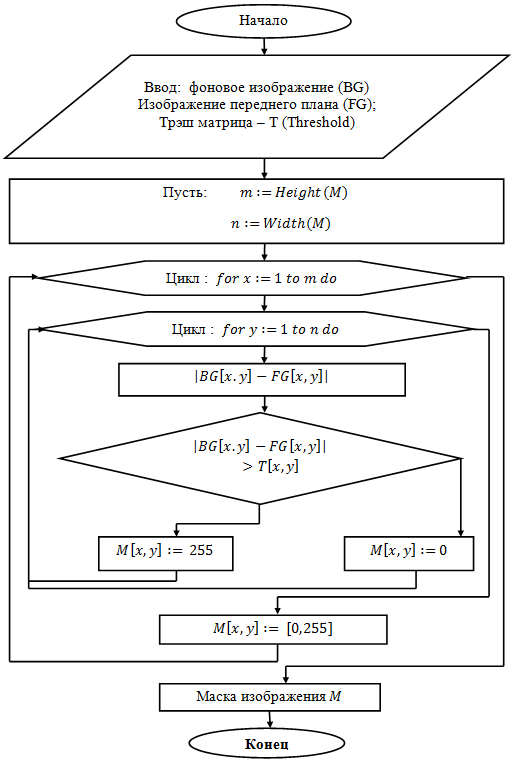
\includegraphics [scale=1] {images/h10.png}
%\captionsetup{justification=justified, labelsep=period}
\caption{Блок-схема алгоритма вычитания фона.} \label{img10}
\end{center}
\end{figure}

\begin{figure}[ht!]
\centering
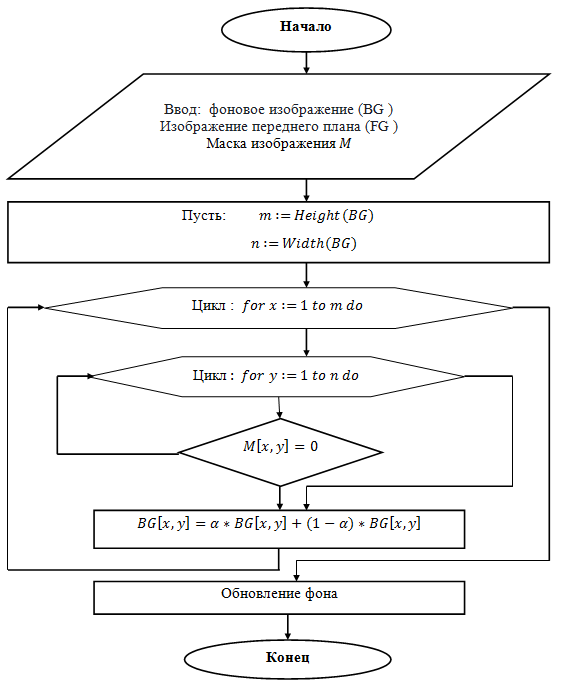
\includegraphics [scale=1] {images/h11.png}
\begin{center}
%\captionsetup{justification=justified, labelsep=period}
\caption{Блок-схема алгоритма обновления фона.} \label{img11}
\end{center}
\end{figure}

Каждый пиксель моделируется как случайный вектор. Значение пикселя $x$ в момент времени $t : x^{\left(t\right)}$. Значения пикселей на основе распределения гауссово смеси:

\begin{equation}\label{eq11}
P\left(0|\theta\right)=\sum^K_{k=1}\pi_kN\left(x|\mu_k,\beta_k\right).
\end{equation}

Для обновления фона в видео, модель фона должна постоянно обновляться, с помощью случайной выборки $X=\left\{x^{\left(t\right)},..., x^{\left(t-T\right)}\right\}$для оценки параметров модели. Метод максимального распределения (Maximize Posteriori) используется для оценки подходящих параметров в гауссовой модели по формуле:
\begin{equation}\label{eq12}
\hat{\theta} = argmax_\theta \left\{\ln p\left(X|\theta\left(K\right)\right)+\ln p\left(\theta\left(K\right)\right)\right\},
\end{equation}
Где:

\begin{itemize}
	\item $K$ параметр модели;
	\item $P\left(\theta\left(K\right)\right)$Функция распределения параметра $\pi\left(K\right)\equiv\left\{\pi_1, ..., \pi_K\right\}$.
\end{itemize}

Согласно \cite{Bishop2006}
\begin{equation}\label{eq13}
\frac{\partial}{\partial\theta}\left\{\ln P\left(X|\theta\left(K\right)\right)+\ln P\left(\theta\left(K\right)\right)+\gamma\left(\sum^K_{k=1}\pi_k-1\right)\right\},
\end{equation}
\begin{equation}\label{eq14}
\longleftrightarrow \frac{\partial}{\partial\theta}\left\{\sum^t_{n=1}ln\left\{\sum^N_{k=1}\pi_kN\left(x^{\left(n\right)}|\mu_k,\beta_k\right)\right\}-\frac{c}{2}\sum^N_{k=1}ln \pi_k + \gamma\left(\sum^K_{k=1}\pi_k-1\right\}\right) = 0,
\end{equation}
Где:
 $c=\frac{N}{2}$, $N$ - каличество параметров для каждой модели компонента \cite{Figueiredo2002}.
\begin{equation}\label{eq15}
\hat{\pi}^{\left(t\right)}_k = \frac{\hat{\pi}^{\left(t\right)}_k\frac{c}{t}}{1-K\frac{c}{t}},
\end{equation}
\begin{equation}\label{eq16}
\mu^{\left(t\right)}_k = \frac{1}{N_k}\sum^t_{n=1}\gamma^{\left(t\right)}\left(z^{\left(n\right)}_k\right)x^{\left(n\right)},
\end{equation}
\begin{equation}\label{eq17}
\beta^{\left(t\right)}_k =\frac{1}{N_k}\sum^t_{n=1}\gamma^{\left(t\right)}\left(z^{\left(n\right)}_k\right)\left(x^{\left(n\right)}-\mu^{\left(n\right)}_k\right)\left(x^{\left(n\right)}-\mu^{\left(n\right)}_k\right)^T.
\end{equation}
Для построения алгоритма обновления фона, необходимо использовать наблюдаемое значение и поэтому предыдущий результат построения обновляется. Уравнение обновления модели описывается следующим образом:
\begin{equation}\label{eq18}
\hat{\pi}^{\left(t+1\right)}_k=\hat{\pi}^{\left(t\right)}_k + \left(t-1\right)^{-1} \left(\frac{\gamma z^{\left(t\right)}_k}{1-K\frac{c}{T}} - \hat{\pi}^{\left(t\right)}_k\right) - \left(1-t\right)^{-1} \frac{\frac{c}{T}}{1-K\frac{c}{T}},
\end{equation}
\begin{equation}\label{eq19}
\hat{\mu}^{\left(t+1\right)}_k = \hat{\mu}^{\left(t\right)}_k + \left(t+1\right)^{-1} \frac{\gamma^{\left(t\right)}z^{\left(t+1\right)}_k}{\hat{\pi}^{\left(t\right)}_k}\left(x^{\left(t+1\right)}-\hat{\mu}^{\left(t\right)}_k\right),
\end{equation}
\begin{equation}\label{eq20}
\hat{\beta}^{\left(t+1\right)}_k = \hat{\beta}^{\left(t\right)}_k + \left(t+1\right)^{-1} \frac{\gamma^{\left(t\right)}z^{\left(t+1\right)}_k}{\hat{\pi}^{\left(t\right)}_k} \left(x^{\left(t+1\right)}-\hat{\mu}^{\left(t\right)}_k\right)\left(x^{\left(t+1\right)}-\hat{\mu}^{\left(t\right)}_k\right)^T - \hat{\beta}^{\left(t\right)}_k.
\end{equation}

Уравнение (\ref{eq18}) строится из (\ref{eq15}) с $\frac{c}{t}=\frac{c}{T}$  с применением гауссовой модели, чтобы обновить модели фона, помочь алгоритму вычитания фона работать быстрее в режиме реального времени и хорошей точности.


